\documentclass[10pt]{article}\usepackage[margin=.65in]{geometry}\usepackage[T1]{fontenc}\usepackage{graphicx}\setlength{\parindent}{0pt}\setlength{\parskip}{6pt}\sloppy\begin{document}{\large Reviewed runtime context staged and checked}\par Observed 2026-11-02. The proposed runtime context is now staged locally with 19 exact members and 10,509,133 file bytes. A separate readback checked the complete member set, SHA-256 digests, byte lengths, types and modes. This closes the previously unstaged-context binding; it is a producer check, not an independent review.\par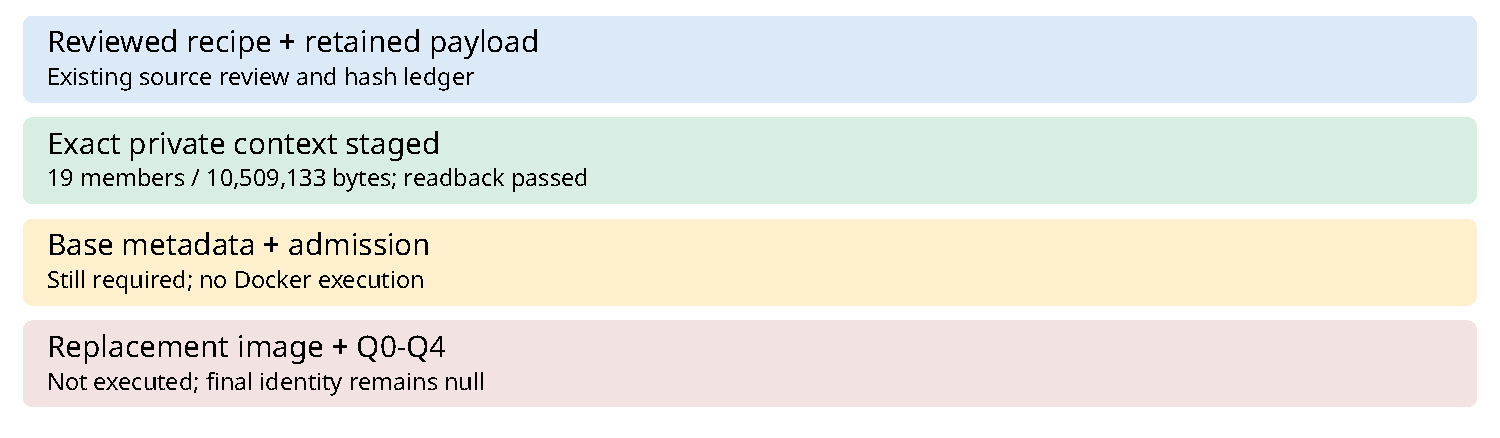
\includegraphics[width=\linewidth]{diagram.pdf}\par Construction. The context combines the 17-member retained payload/placeholder ledger, one explicit mountpoints directory and the independently reviewed Dockerfile. All 15 original runtime members and both empty placeholder files matched the retained source identities. The private enclosing directory is 0700, context root 0755; file and directory modes are recorded individually. The staging script validates input hashes before writing and creates a fresh directory. It assumes trusted source ancestors and a single writer; it does not claim protection against concurrent hostile mutation.

Identity. Recipe SHA-256: 5d86b44b9f087a430969c40882db60127d4fcfdb5934bb87cc4d2398dbcec21b. Exact local path and every member digest are in staging-receipt.json. readback.json binds that receipt. Runtime binaries remain in the private local context; their existing custody references remain in the earlier binding packet. Restaging requires those exact source bytes and creates a new receipt; no payload is executed by stage.py.

Preserved result. The historical qualification passed Q0 and failed Q1 after the diagnostic exited zero because Docker reported additions at /fixtures, /qualification and /qualification/exec-gate. Cleanup completed. The reviewed COPY amendment is intended to pre-create the mount destinations; its runtime effect is still untested. Neither the failed receipt nor the strict empty-diff acceptance check was changed.

Next binding. Inspect ancestor path types, modes and ownership in the exact base image under a bounded admitted method. Then complete assembler and qualifier bindings, independent prospective review and execution admission. The base identity in the earlier ledger is historical, not freshly inspected here. New image identity and qualification receipt remain null. Docker operations, cloud actions, payload executions and scientific trials in this step: zero.

Campaign scope. The new planning allowance is 25,200 active-worker seconds with absolute deadline 2026-11-03 06:00 UTC; prior campaign records are unchanged. The full cohort remains 1,260 targets and 22,680 planned executions including warmups. This software preparation neither initializes remaining scientific allowance nor supplies missing campaign accounting. Independent review agents currently report usage-limit failures.

Sources and validation. Read runtime-mountpoint-review/REPORT.md, runtime-binding-reconciliation/evidence/proposed-context-member-ledger.json and runtime-outcome/status.json. Docker COPY and ONBUILD documentation: https://docs.docker.com/reference/dockerfile/. Context modes matter to COPY; inherited base instructions and ancestor metadata remain separate checks. No scientific comparison was performed, so the diagram shows binding stages rather than a cost graph. Canonical scientific graphs are unchanged. The earlier root Rust release checks remain failed allocation / timed out; this change only stages files and adds packaging scripts.
\end{document}